%!TEX root = "../../../DA_GUI.tex"

%	--------------------------------------------------------
% 	Debugger: Einleitung
%	--------------------------------------------------------

\section{Einleitung}

%   --------------------------------------------------------
%   Grundlegende Funktionen, Ideen
%   --------------------------------------------------------

\subsection{Die grundlegende Idee}
Ein wichtiger Bestandteil von C Compact ist der integrierte Debugger, der speziell für die Bedürfnisse von Anfängern ausgelegt ist. Während das Programm Schritt für Schritt abgearbeitet wird, sind alle Variablen und der Call Stack in übersichtlicher Form dargestellt. In der Variablentabelle werden Wertänderungen farbig hervorgehoben. Dadurch soll ein fundiertes Verständnis für den Programmablauf und die Logik dahinter entstehen.

\begin{figure}[h]
\centering
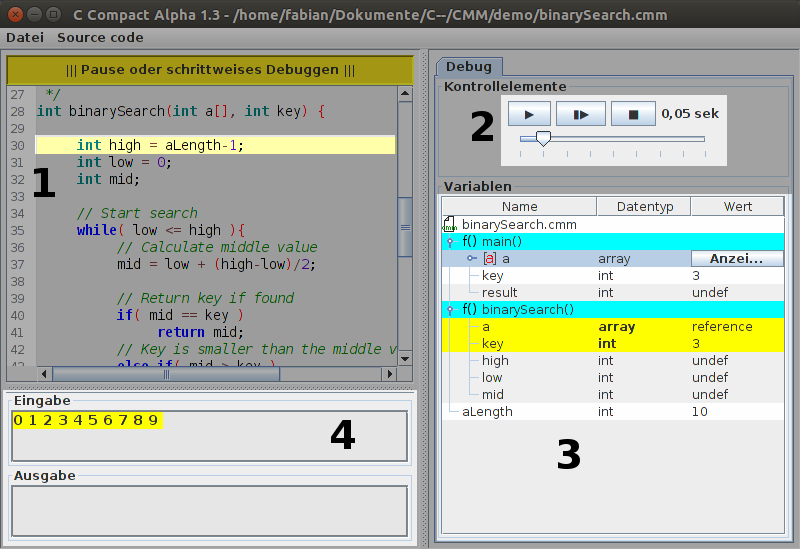
\includegraphics[width=0.7\textwidth]{./media/images/gui/debugger/gui-debugger-marked.png}
\caption{Die vier Komponenten des Debuggers}
\label{fig:deb-intro-m1}
\end{figure}

Während die Debugger professioneller Entwicklungsumgebungen eine Hilfestellung für erfahrene Programmierer sind, ist der Debugmodus von C Compact besonders auf Anfänger ausgelegt. Damit Einsteiger und unerfahrene Programmierer von Beginn an mit dem Debugger in Berührung kommen, ist er ein fester Bestandteil der Benutezroberfläche.

Abbildung \ref{fig:deb-intro-m1} zeigt die vier Komponenten des Debuggers in der Benutzeroberfläche:
\begin{enumerate}
\item Im Quelltext wird die gerade abgearbeitete Zeile markiert
\item Mit den Kontrollelementen kann der Debugger gestartet und angehalten werden
\item Die Variablen des Programmes werden übersichtlich angezeigt
\item Ein- und Ausgabe des laufenden Programmes befinden sich in getrennten Textfeldern, eingelesene Zeichen werden gelb markiert.
\end{enumerate}

%TODO somewhere else:
% Fehler im Präprozessor, Compiler oder Interpreter werden dem Benutzer übersichtlich angezeigt und verständlich erklärt. Außerdem werden Hinweise zur Fehlersuche und -behebung gegeben.
%TODO ref: nicht verwechseln mit internen Fehlern

%   --------------------------------------------------------
%   Bedienung des Debuggers
%   --------------------------------------------------------

\subsection{Bedienung des Debuggers}

Mit den Kontrollelementen kann der Debugger intuitiv und einfach bedient werden. Die Bedienelemente (Abbildung \ref{fig:deb-gui-ctrl}) sind im rechten Teil des Hauptfensters im Tab \glqq{}Debug\grqq{} (Siehe Kapitel \ref{sec:gui-main-right-reg-deb}) zu finden.

\def\arraystretch{1.4}
\begin{table}[h]
\begin{tabular}{|l|l|l|l|}
	\hline
	Element & \parbox{2cm}{Keyboard\\Shortcut}& Name & Funktion\\
	\hline
	\ding{228} / \ding{122}\thinspace \ding{122} & F5 & Play/Pause & Startet den Debugger/Hält den Debugger an\\
	\ding{122}\thinspace \ding{228} & F6 & Step & Springt zum nächsten Schritt weiter\\
	\ding{110} & F7 & Stop & Beendet den Debugger\\
	--- & --- & Schieberegler & \parbox{7cm}{Ändert die Zeitabstände beim automatischen Abarbeiten}\\
	\hline
\end{tabular}
\caption{Funktionen der Bedienelemente des Debuggers}\label{tab:deb-ctrl}
\end{table}



\begin{figure}[h]
\centering
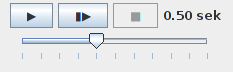
\includegraphics[width=0.4\textwidth]{./media/images/gui/debugger/ctrl-elements.png}
\caption{Kontrollelemente des Debuggers}
\label{fig:deb-gui-ctrl}
\end{figure}

Der Debugger hat vier unterschiedliche Modi, diese wurden bereits in Kapitel \ref{sec:gui-main-left-zust} überblicksmäßig beschrieben. Der Wechsel zwischen diesen Zuständen erfolgt durch Eingaben des Benutzers, entweder mit den Kontrollelementen (Buttons) in der Benutzeroberfläche, oder mit Keyboard Shortcuts.
%TODO ref keyboard shortcuts

Die vier Zustände sind:
\begin{enumerate}
\item \textbf{Text bearbeiten (ready mode)}
Dies ist der Standardzustand. Der Quelltext und Eingabedaten für den Debugger können bearbeitet werden. Außerdem sind Dateioperationen erlaubt.
\begin{figure}[h!]
\centering

\includegraphics[width=0.65\textwidth]{./media/images/gui/debugger/mode-idle.png}
\caption{Zustandsanzeige für den Editormodus}
\label{fig:deb-zust-1}
\end{figure}
\item \textbf{Fehler aufgetreten (error mode)}
Beim Compilieren oder während der Laufzeit des Debuggers ist ein Fehler aufgetreten. Um diesen zu beheben, ist das Bearbeiten des Quelltexts nach wie vor erlaubt.
\begin{figure}[h!]
\centering

\includegraphics[width=0.65\textwidth]{./media/images/gui/debugger/mode-error.png}
\caption{Zustandsanzeige für den Fehlermodus}
\label{fig:deb-zust-2}
\end{figure}
\item \textbf{Programm Schritt für Schritt abarbeiten oder Pause (pause mode)}
Der Debugger ist aktiv, wartet aber auf eine Eingabe des Benutzers, um den nächsten Befehl abzuarbeiten. In diesem Modus kann der Benutzer sein Programm Schritt für Schritt abarbeiten. Das Modifizieren des Quelltextes ist in diesem Modus nicht möglich.
\begin{figure}[h!]
\centering

\includegraphics[width=0.65\textwidth]{./media/images/gui/debugger/mode-step.png}
\caption{Zustandsanzeige für den Pausemodus}
\label{fig:deb-zust-3}
\end{figure}
\item \textbf{Programm automatisch abarbeiten (run mode)}
Das Programm des Benuters wird Schritt für Schritt abgearbeitet. Zwischen den Befehlen wird für eine bestimmte Zeit zwischen 0 und 5 Sekunden gewartet. Diese Verzögerung kann mit dem Schieberegler bei den Kontrollelementen eingestellt werden. Auch hier kann der Quelltext nicht verändert werden.
\begin{figure}[h!tp]
\centering

\includegraphics[width=0.65\textwidth]{./media/images/gui/debugger/mode-run.png}
\caption{Zustandsanzeige für den Automatischen Debugmodus}
\label{fig:deb-zust-4}
\end{figure}
\end{enumerate}

\begin{figure}[h]
\centering
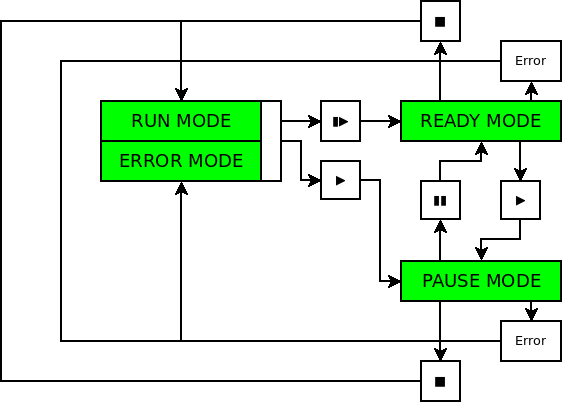
\includegraphics[width=0.65\textwidth]{./media/images/gui/debugger/RunModes_Simple.png}
\caption{Vereinfachtes Zustandsdiagramm des Debuggers}
\label{fig:deb-zust-simple}
\end{figure}

Obwohl der Debugger selbst zwischen Modus Editormodus (1) und Fehlermodus (2) unterscheidet, gibt es in der Benutzeroberfläche nur mehr den Editormodus. Der Fehlermodus wird trotzdem im Zustandspanel des Debuggers im Hauptfenster angezeigt, damit der Benutzer auf den aufgetretenen Fehler aufmerksam gemacht wird. Wie in Abbildung \ref{fig:deb-zust-simple} ersichtlich ist, erfüllen die beiden Modi die selben Funktionen.

Der Pausemodus (3) hat zwei Funktionen: einerseits entspricht dieser Modus einer Pausierung (bezogen auf Zustand 4, in dem der Debugger automatisch durchläuft) und andererseits kann in diesem Modus mit dem mittleren Button auch direkt zum nächsten Schritt gesprungen werden.

Ein Sonderfall des run mode ist der \glqq{}quick run mode\grqq{}. Wenn der Regler für die Zeitabstände zwischen den Schritten des Debuggers auf null gestellt wird, werden die folgenden Schritte so schnell wie möglich abgearbeitet, bis entweder das Programm zu Ende ist oder der Debugger auf einen \glqq{}wait\grqq{}-Befehl stößt (Siehe Kapitel \ref{}).

%TODO ref commands

%   --------------------------------------------------------
%   Schlüsselwörter
%   --------------------------------------------------------

\subsection{Schlüsselwörter}
%TODO ref compiler
%TODO ref panelRunListener
In der Sprache von C Compact gibt es zwei spezielle Schlüsselwörter, die Einfluss auf das Verhalten des Debuggers nehmen: \textbf{wait} und \textbf{library}.

\subsubsection*{wait}
%TODO ref AST
%TODO check version number, ref versions
In C Compact gibt es seit der Verion 1.2 keine Breakpoints als Option in der Benutzeroberfläche mehr. Anstatt dessen wird der Befehl \textbf{wait} verwendet. Dieser Befehl kann in jeder Funktion verwendet werden. Stößt der Debugger diesen Befehl, geht er in den \textbf{Pausemodus}. An dieser Stelle kann der Debugger dann entweder Schritt für Schritt, oder wieder im automatischen Debugmodus fortgesetzt werden.

\begin{lstlisting}[language=CMM]
wait;
\end{lstlisting}

Durch die Umsetzung der Breakpoint-Funktion als Befehl in der Sprache besteht immer ein klarer Zusammenhang zwischen Aktionen des Debuggers und dem Quelltext.

\subsubsection*{library}
%TODO read this paragraph
Funktionen und Variablen können vor dem Debugger \glqq{}versteckt\grqq{} werden. Das Attribut \textbf{library} kann sowohl für eine Variable, als auch für eine Funktion verwendet werden. Das Schlüsselwort muss immer zwischen Typ und Name der Variable bzw. Funktion stehen.

\begin{lstlisting}[language=CMM]
const float library M_PI = 3.141592654;
\end{lstlisting}
Eine Variable mit dem \textbf{library}-Attribut wird im Debugger nicht angezeigt. Dies wird zum Beispiel verwendet, um die zahlreichen Konstanten der Bibliothek \textbf{math.h} im Debugger auszublenden.

\begin{lstlisting}[language=CMM]
float library sin(float x);
\end{lstlisting}
Hat eine Funktion das \textbf{library}-Attribut, springt der Debugger nicht in diese Funktion, sondern arbeitet sie in einem Schritt ab. Dadurch können Bibliotheksfunktionen im Debugger als Befehl in einem Schritt abgearbeitet werden.
